\documentclass[10pt,twocolumn,letterpaper]{article}
\usepackage{cvpr}
\usepackage{times}
\usepackage{latin1}
\usepackage{epsfig}
\usepackage{graphicx}
\usepackage{amsmath}
\usepackage{amssymb}
\usepackage[utf8]{inputenc} 
\usepackage[breaklinks=true,bookmarks=false]{hyperref}
\usepackage{epstopdf}
\cvprfinalcopy % *** Uncomment this line for the final submission
\def\cvprPaperID{****} % *** Enter the CVPR Paper ID here
\def\httilde{\mbox{\tt\raisebox{-.5ex}{\symbol{126}}}}

% Pages are numbered in submission mode, and unnumbered in camera-ready
%\ifcvprfinal\pagestyle{empty}\fi
\setcounter{page}{1}
\begin{document}

%%%%%%%%% TITLE
\title{Evaluación de la precisión y sensibilidad de dos métodos de agrupamiento: K-means y GMM, entrenándolos con el software Matlab.}

\author{David L. Henao\\
\begin{normalsize}
Grupo de Ingeniería Biomédica. Universidad de los Andes, Bogotá, Colombia
\end{normalsize}
\\
{\tt\small dl.henao909@uniandes.edu.co}}
% For a paper whose authors are all at the same institution,
% omit the following lines up until the closing ``}''.
% Additional authors and addresses can be added with ``\and'',
% just like the second author.
% To save space, use either the email address or home page, not both
\maketitle
%\thispagestyle{empty}

%%%%%%%%% ABSTRACT
\begin{abstract}

En el siguiente artículo se presenta la metodología desarrollada para crear una función que realiza segmentación de imágenes con algoritmos de agrupamiento. Esta se realizó, empleando métodos de clasificación no supervisada conocidos en la actualidad. Dichos métodos, que incluyen kmeans, mezcla de matrices gaussianas (GMM) y líneas divisoras de agua (watersheds)fueron implementados en los diferentes espacios de color RGB,HSV y LAB. Así mismo, se presentan los resultados evaluativos de la sensibilidad y la precisión de dos de estos métodos, particularmente kmeans y GMM. Estos resultados se obtuvieron entrenando la función en el espacio RGB con una base de datos de 200 imágenes y realizando una comparativa con 200 imágenes de prueba. Si bien los resultados no son los mejores teniendo en cuenta los métodos actuales de segmentación, nos permiten realizar una primera cuantificación del comportamiento de la función creada.
   
\end{abstract}

%%%%%%%%% BODY TEXT
\section{Introducción}

El agrupamiento de datos, hace referencia al proceso de juntar datos similares en el mismo "cluster" (grupo) o dividir datos no similares en diferentes grupos de acuerdo a algunos criterios previamente definidos. Aparentemente, los métodos desarrollados para resolver el problema de agrupamiento, pueden ser fácilmente aplicados y extendidos a diferentes dominios como el análisis de documentos, análisis finaciero y la bio-información. En la actualidad, muchos investigadores han adoptado diferentes aproximaciones para resolver el problema de agrupamiento las cuales incluyen k-means y support vector machine [1]. Siendo conocido kmeans y sus variaciones como algoritmos rápidos de agrupamiento [2].

K-means es un método de clasificación no supervisada en donde se asume que el número de klusters k es conocido y los elementos son puntos en $\mathbb{R}$n. El método consiste en representar cada cluster por su centroide y minimizar las distancias cuadradas entre elementos y centroides. Para ello se emplea el algoritmo de Lloyd:

\begin{itemize}
\item Se seleccionan k centroides aleatoreamente.
\item Se asignan los elementos de la imagen a cada grupo definido por los centroides (diagrama de Voronoi).
\item Se re calculan los centroides de acuerdo a dicha asignación.
\item Se repiten los dos pasos anteriores hasta que el algoritmo converja.
\end{itemize}

Por otro lado, en el enfoque de la segmentación de imágenes que típicamente se puede dividir en agrupamiento espectral y agrupamiento suave, el éxito del primero está comprometido cuando las imágenes están altamente corrompidas con ruido, valores atípicos y demás artefactos comunes. En este sentido, los algoritmos de agrupamiento suave han demostrado obtener buenos resultados en la segmentación de imágenes pues a cada pixel de la imagen se le permite pertenecer a más de un grupo. Esto, asociando un nivel de pertenencia que indica la fuerza de las asociaciones entre pixeles y grupos[3]. Este es el caso del modelo de mezclas de Gaussianas el cual, al generar una probabilidad normal a cada asociación nos permite un comportamiento más robusto en la clasificación respecto al ruido y los valores atípicos de la imagen.

De esta manera, en el método de mezclas de gaussianas, no se representa cada grupo por el centroide sino por una distribución gaussiana. Reemplazando así la distancia euclídea por la distancia de Mahalanobis que tiene en cuenta la distribución de los datos[4].
\begin{equation}
p (x|\{\pi_k,\mu_k,\Sigma_k\})=\Sigma \pi_k N (x|\mu_k,\Sigma_k)
\end{equation}

Donde:\\

$N (x|\mu_k,\Sigma_k)$ Representa a las distribuciones Gaussianas y $\pi_k$ los coeficientes de mezcla.\\

El algoritmo empleado para realizar la clasificación GMM es el algoritmo de esperanza-maximización[4]:
\begin{itemize}
\item Se estiman las responsabilidades de los elementos. Es decir "Pertenezco al grupo 1 en un 0.7 y al grupo 2 en 0.3.
\item Se estiman los parámetros teniendo las responsabilidades..
\end{itemize}

En el presente artículo, se presenta la metodología llevada a cabo durante la clase de laboratorio, en la que se desarrollo y entrenó una función que realiza segmentación de imágenes empleando los métodos de kmeans, mezcla de matrices gaussianas y línea divisora de aguas para los espacios de color RGB, HSV y LAB. Se realiza una evaluación de dicha función en el espacio de color RGB para los primeros 2 métodos. Así mismo, como resultado cualitativo de la función, se construyeron las respectivas curvas de sensibilidad vs precisión empleando una base de datos de test de 200 imágenes.

%------------------------------------------------------------------------
\section{Metodología}

Para construir la función de segmentación "henao\_segment\_clustering", primero se definieron los métodos de agrupamiento a incluir y los espacios de color para cada método. Se muestra el resumen de dichas combinaciones en la figura 1.Luego,se escribieron tantas funciones individuales como número de combinaciones posibles entre método de agrupamiento y espacio de color. Obteniendo de esta manera un total de 15 scrips individuales en forma de función, cada uno de ellos tiene como entrada el nombre de una imagen en formato RGB y el número de clusters en los que se quiere segmentar la imagen.

\begin{figure}[t]
\begin{center}
%\fbox{\rule{0pt}{2in} \rule{0.9\linewidth}{0pt}}
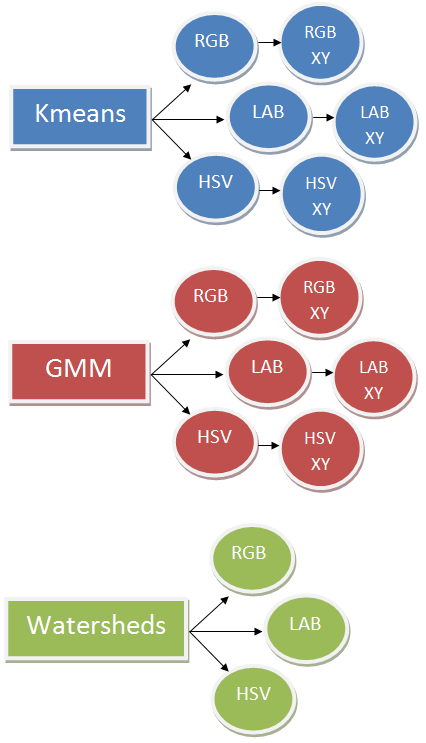
\includegraphics[width=0.6\linewidth]{Esquema_fun.png}
\end{center}
   \caption{Esquema de los métodos y espacios de color de la función "henao\_segment\_clustering".}
\label{fig:seg}
\end{figure}

En la figura 2, se puede observar una imagen de muestra que se empleó para probar (más no evaluar) el funcionamiento de las funciones de segmentación programadas.

\begin{figure}[t]
\begin{center}
%\fbox{\rule{0pt}{2in} \rule{0.9\linewidth}{0pt}}
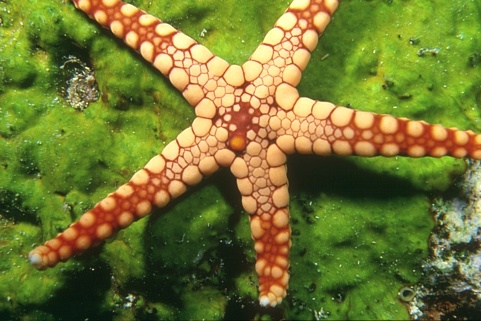
\includegraphics[width=0.6\linewidth]{12003.jpg}
\end{center}
   \caption{Imagen de prueba empleada en las funciones escritas.}
\label{fig:seg}
\end{figure}


\subsection{Construcción de la función de clasificación}

Para crear las funciones que realizan la segmentación empleando el método de kmeans, primero se lee la imagen y dependiendo si se requiere realizar la clasificación en RGB o un espacio de color diferente (LAB o HSV) se debe convertir dicha matriz al respectivo espacio de color empleando las funciones nativas de Matlab. Una vez que se tiene la matriz de la imagen en el espacio de color requerido, se debe redimensionar la misma del espacio mxnx3 a m*nx3. Obtenido este redimensionamiento, se procede a aplicar la función kmeans incluida en las librerías de MATLAB la cual, al ingresar la matriz creada y el número de clusters deseados retorna el vector de segmentación que a su vez se vuelve a redimensionar al tamaño de la matriz nxm para graficar los resultados de la segmentación.

En el caso de los espacios de color RGBxy, LABxy y HSVxy se implementan en sus respectivas funciones un recorrido adicional que guarda en dos vectores las coordenadas en pixeles de cada pixel de la imagen y se introducen dichos vectores como columnas adicionales en la matriz creada. Esto debido a que en estos espacios se tendrán en cuenta adicional al espacio de color, la posición entre pixeles para la segmentación.

Respecto a la segmentación empleando el método de GMM: Se lee la imagen y dependiendo si se requiere realizar la clasificación en RGB o un espacio de color diferente (LAB o HSV) se convierte dicha matriz al espacio de color deseado. Una vez que se tiene la matriz de la imagen en el espacio de color requerido, se convierte al formato "double" y se redimensiona de la misma manera que con el método de kmeans. Luego, se procede a crear la distribución gaussiana regularizada al 0.001 y con ésta, el número de clusters y la matriz anteriormente mencionada se crea el vector de segmentación que nuevamente se vuelve a redimensionar al tamaño de la matriz nxm para graficar los resultados de la segmentación.

En el caso de los espacios de color RGBxy, LABxy y HSVxy para el método de segmentación GMM se realiza el mismo procedimiento que con el método kmeans.

Por otro lado, para los algoritmos de línea divisora de aguas watersheds se realiza una conversión al espacio de color deseado. Luego se vuelve a convertir la imagen, esta vez a escala de grises y al formato double para posteriormente hallar las derivadas parciales df/dx y df/dy implementando sobre la imagen un filtro "sobel" y su transpuesta. Con las derivadas parciales se halla el gradiente definido como la raíz cuadrada de la suma de las derivadas parciales.

Con el gradiente y la altura de la superficie que desee el usuario, se hallan y se extienden los mínimos regionales de la imagen empleando las funciones imextendedmin y imimposemin. Finalmente se realiza la función de línea divisora de aguas a los mínimos extendidos, se redimensiona el vector resultante para poder graficarlo y ver los resultados de la segmentación. En la figura 3, se puede observar una segmentación realizada con este algoritmo a la imagen de muestra de la figura 2 con una altura de mínimos extendidos de 30.

\begin{figure}[t]
\begin{center}
%\fbox{\rule{0pt}{2in} \rule{0.9\linewidth}{0pt}}
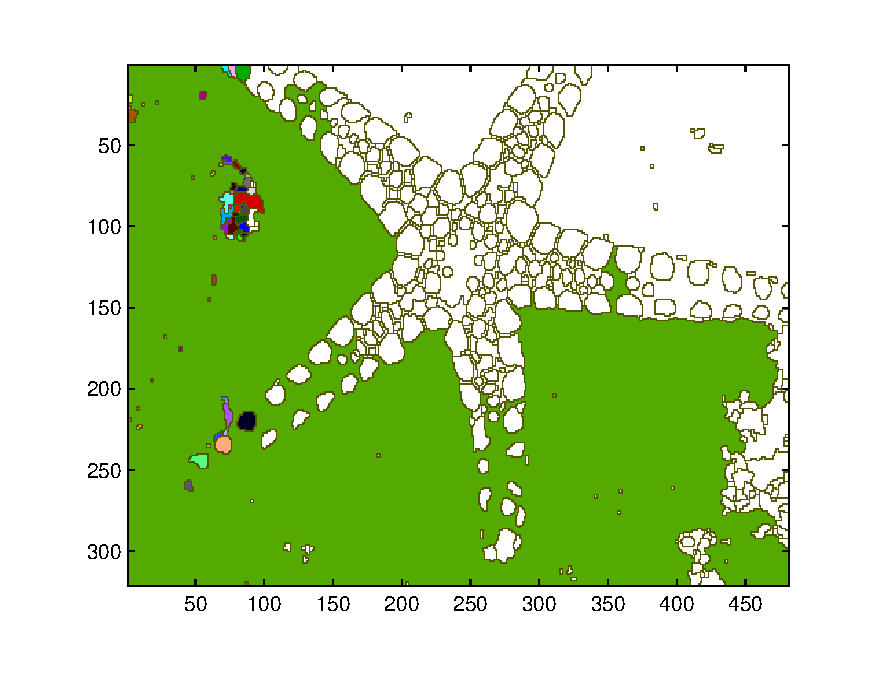
\includegraphics[width=0.8\linewidth]{estrellaWS30.eps}
\end{center}
   \caption{Segmentación de la imagen de prueba empleando el algoritmo de watersheds con h=30.}
\label{fig:seg}
\end{figure}

Finalmente, se construyó la función "henao\_segment\_clustering" la cual de acuerdo a los parámetros de método de segmentación y espacio de color seleccionados, llama a una de las 15 funciones creadas y entrega como resultado el vector de segmentación.
%-------------------------------------------------------------------------
\subsection{Prueba de la función de clasificación}

Para poder probar la precisión y sensibilidad de la función creada, primero se seleccionaron dos métodos de segmentación y un espacio de color sobre los que se realizaría dicha evaluación. Esto debido a los costos computacionales de cada evaluación y a que para algunas combinaciones de método - espacio de color no se obtenían los mejores resultados visuales. Por ejemplo para el caso de la segmentación Kmeans con dos clusters en los espacios de color LABxy o RGBxy se divide la imagen en dos regiones horizontal y verticalmente sin tener en cuenta el contenido de la misma. De esta manera se seleccionaron los métodos de Kmeans y GMM en el espacio de color RGB para ser evaluados.

Una vez seleccionados dichos métodos y espacios de color, se realizó un entrenamiento de la función para los mismos. Este se implemento tomando 200 imágenes de entrenamiento de una base de datos. Se segmentó cada una de estas imágenes para Kmeans y GMM con 2,4,6,8 y 10 clusters y los resultados de cada segmentación fueron guardados en una celda de dimensión 5. Cada una de estas celdas a su vez en un archivo salvado como nombredelaimagen.mat

Ahora, para construir la gráfica de precisión y sensibilidad  se realizaron 1000 segmentaciones para cada método (200 imágenes y 5 clusters) y se implementó la función bench.m disponible en los repositorios de GitHub del curso. Dicha función tomaba una base de datos de 200 imágenes de prueba y evaluaba con esta la función entrenada con las 2000 segmentaciones. 

\section{Resultados}

\subsection{kmeans en diferentes espacios de colores}

En la figura 4, se muestran los resultados de la segmentación para Kmeans en todas las combinaciones de método - espacio de color creadas. Para obtener esta imagen, se realizó una segmentación con 2 clusters para cada espacio de color y como se puede observar, los mejores resultados se obtienen en los espacios de color que no tienen en cuenta la posición xy para realizar la segmentación. Esto probablemente se deba a que la geometría a segmentar es simétrica y al añadir como entrada la posición de los pixeles se tiende a dividir el espacio horizontal o verticalmente de acuerdo a las características del espacio de color (Saturación, matiz, valor, brillo, luminosidad) y no a la geometría de la imagen. En este sentido, cualitativamente los resultados que más se acercan a la segmentación de la geometría fueron los obtenidos por Kmeans en los espacios RGB y HSV.

\begin{figure}[t]
\begin{center}
%\fbox{\rule{0pt}{2in} \rule{0.9\linewidth}{0pt}}
   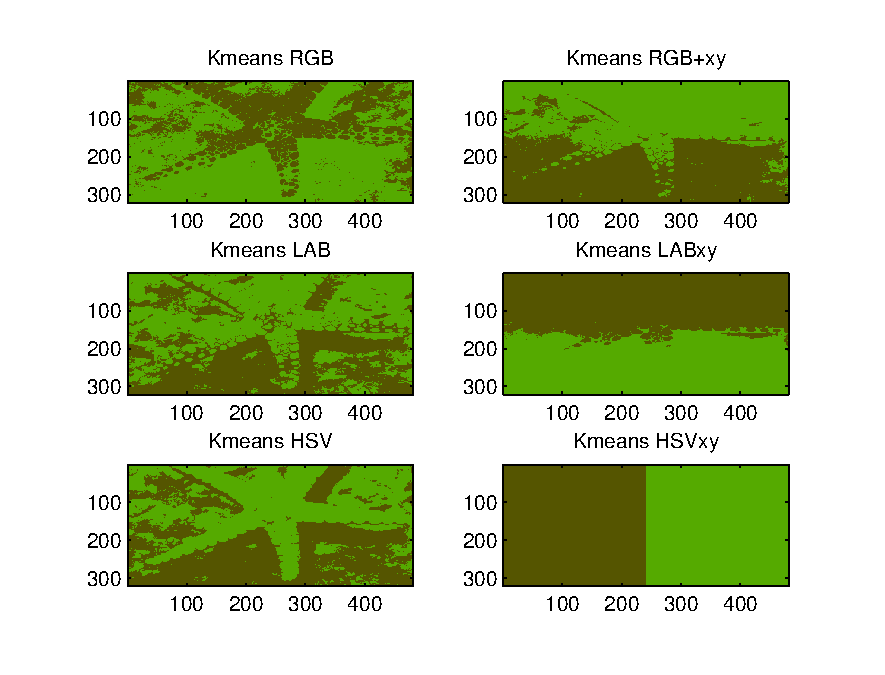
\includegraphics[width=1\linewidth]{seg_colorspace.eps}
\end{center}
   \caption{Segmentaciones sobre la imagen de prueba con Kmeans en los espacios de color:(a) RGB(b) RGBxy (c)LAB (d)LABxy (e) HSV (f) HSVxy }
\label{fig:seg}
\end{figure}

\subsection{GMM en diferentes espacios de colores}

Por su parte, en la figura 5 se muestran los resultados de la segmentación para GMM en todas las combinaciones de método - espacio de color creadas. Para obtener esta imagen, se realizó una segmentación con 2 clusters para cada espacio de color y como se puede observar, los resultados son congruentes en todos los espacios de colores. Cuando se tiene en cuenta la posición para producir la segmentación el algoritmo GMM permite a la distancia adaptarse a la distribución de datos por lo que a pesar de que la geometría a segmentar es simétrica, al añadir como entrada la posición de los pixeles prima la distribución gaussiana de cada grupo en la geometría de la imagen. Ahora bien, a pesar de los resultados son muy similares para cada uno de los espacios, se logra tener una buena aproximación cualitativamente hablando en los espacios de color RGB, RGBxy, LAB y LABxy.

\begin{figure}[t]
\begin{center}
%\fbox{\rule{0pt}{2in} \rule{0.9\linewidth}{0pt}}
   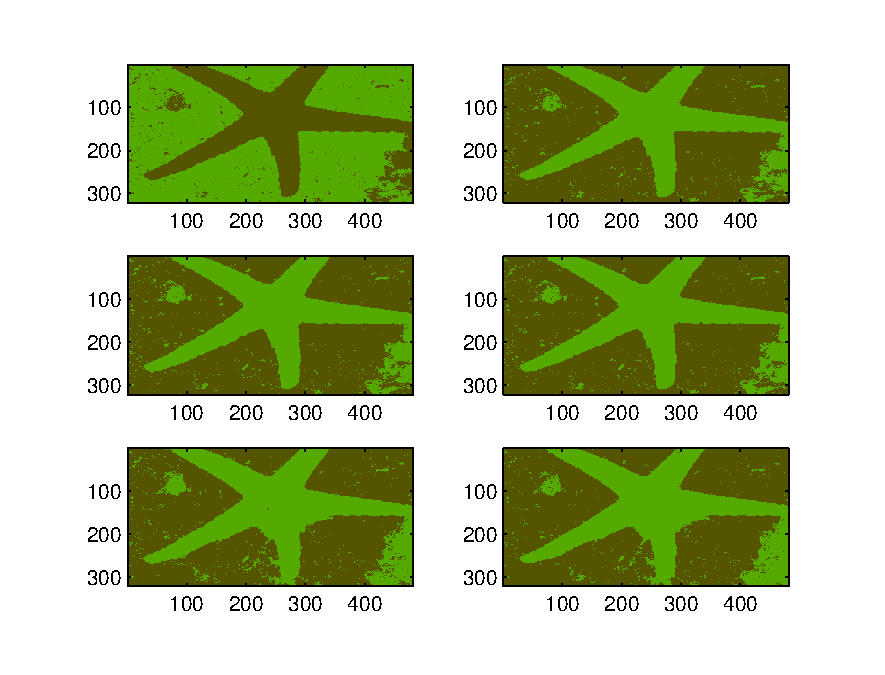
\includegraphics[width=1\linewidth]{seg_colorspacegmm.eps}
\end{center}
   \caption{Segmentaciones sobre la imagen de prueba con GMM en los espacios de color:(a) RGB(b) RGBxy (c)LAB (d)LABxy (e) HSV (f) HSVxy }
\label{fig:seg}
\end{figure}

\subsection{Curva de precisión y sensibilidad}

Para construir la gráfica de precisión y sensibilidad una vez trascurrido el tiempo computacional en el que se completaron las 2000 segmentaciones, se tomaron 200 imágenes de prueba y como resultado se presentan en la figura 6 las curvas de precisión y sensibilidad obtenidas para Kmeans y GMM.

\begin{figure}[t]
\begin{flushleft}
%\fbox{\rule{0pt}{2in} \rule{0.9\linewidth}{0pt}}
   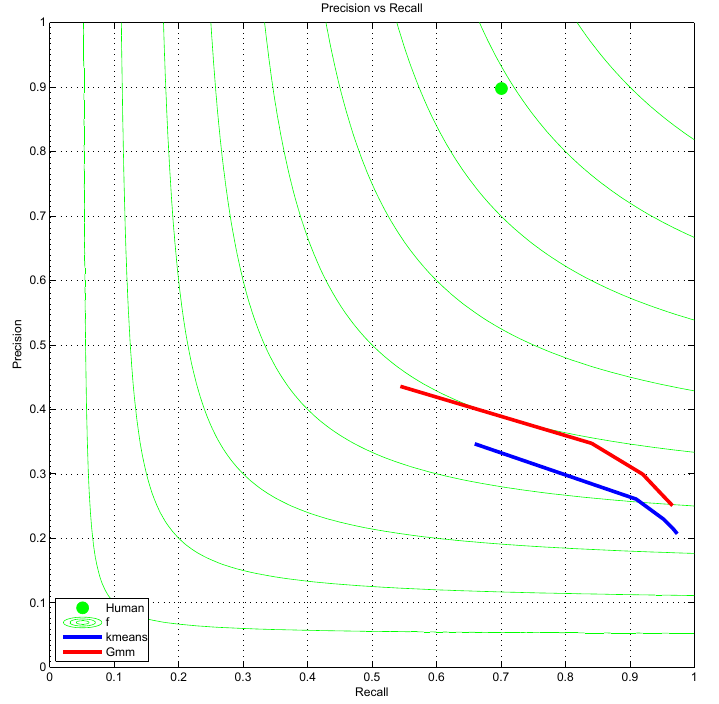
\includegraphics[width=1.1\linewidth]{graf_P_R}
\end{flushleft}
   \caption{Curvas de precisión y sensibilidad obtenidas para Kmeans y GMM con 2,4,6,8 y 10 clusters.}
\label{fig:seg}
\end{figure}

\section{Discusión}

Respecto a los resultados obtenidos para la segmentación de imágenes no supervisada en los diferentes espacios de color para Kmeans y mezcla de gaussianas GMM, se puede observar una ventaja de la segmentación realizada por mezcla de gaussianas respecto a la de kmeans. 

Este fenómeno se puede explicar debido a que Kmeans tiende a formar grupos esféricos alrededor de los centroides de inicialización por lo que en el momento de realizar la segmentación de las imágenes, para geometrías complejas o irregulares no suele tener el mejor desempeño pues sólo tiene en cuenta la distancia euclídea entre los elementos y sus centroides.

Por otro lado, dichos grupos suelen ser del mismo tamaño por lo que para geometrías con regiones a diferentes escalas la segmentación no suele ser la más efectiva y depende de la inicialización de los centroides el desempeño del algoritmo pues puede converger a mínimos locales y detener el proceso iterativo en regiones indeseadas. 

Por su parte la mezcla de matrices gaussianas corrige el efecto de los grupos esféricos del mismo tamaño al permitir que un elemento pertenezca a diferentes grupos representándolo por la distancia de mahalanobis (distribuciones gaussianas). Esto se puede observar en las imágenes segmentadas en donde con GMM los clusters formados son mas uniformes con las regiones propias de la imagen y no con las regiones formadas por la aleatoriedad de los centroides iniciales. Sin embargo, esta forma de agrupamiento no corrige el problema de los mínimos locales pues a pesar de cambiar la representación del cluster y la distancia de cada elemento al mismo, sigue dependiendo de la inicialización de cada grupo.

Una limitación adicional de la segmentación empleando GMM es que se asume una distribución normal de los datos por lo que si bien es un algoritmo menos sensible a ruidos y valores atípicos se pudo observar en las imágenes que si los datos no se distribuían normalmente no se obtienen los resultados esperados.

En la curva de precisión y sensibilidad podemos  observar como GMM se presenta una mayor cobertura sobre el algoritmo de Kmeans. Este resultado se esperaba en el sentido de que para explicar las asociaciones de los elementos a los grupos, en Kmeans se debe modificar la media de la distribución constantemente durante el proceso iterativo lo que hace el algoritmo más sensible al ruido, los valores atípicos y en general a los cambios significativos entre elementos a distancias similares. En el caso del algoritmo de mezclas de gaussianas, este permite establecer la media en un valor fijo y simplemente modificar la relación entre los elementos y los grupos a los que pertenecen como una distribución normal.

Las limitaciones para ambos algoritmos además de las mencionadas con anterioridad, radican en que es necesario dar a la máquina en la etapa de entrenamiento el número de clusters en los que se desea segmentar la imagen, además de que GMM sigue teniendo una sensibilidad al ruido a pesar de que es menor que en kmeans.

Por otro lado, respecto a la función watersheds líneas divisoras de agua, se obtuvieron segmentaciones con poca calidad. Primeramente, se debe mencionar al respecto que la altura de los mínimos extendidos de este algoritmo no es directamente el número de clusters de la imagen tal como se presentan en otros algoritmos de clasificación jerárquica en donde existe una relación con la distancia paramétrica. Por este motivo, cuando se realizaba el proceso de segmentación con valores de h de 2, 4, 6, 8 y 10. El agrupamiento de los datos era mínimo y no se podía observar una buena segmentación. Adicionalmente, existen regiones dentro de dos o más clusters que comparten características similares dentro del espacio de color trabajado esto ocasiona que la altura de los mínimos extendidos sea la misma y cuando se realiza el agrupamiento se pierden la división entre las regiones de interés. Por ejemplo en el caso de la estrella (figura 3), existen regiones dentro de la misma que están a la misma altura de las regiones externas por lo que al realizar la inundación con un h grande, estas dos regiones se agrupan. Además si se realiza una segmentación con alturas menores, se crea una imagen sobresegmentada al unir grupos pequeños que no es de nuestro interés hallar.

Finalmente, para mejorar la función implementada, se propone:

Realizar diferentes inicializaciones aleatorias de los clusters (teniendo en cuenta que los clusters se encuentren dentro de los elementos de la imagen)de manera individual. Y seleccionar la inicialización en la que converjan mejor todos los elementos de la imagen, empleando para ello un indicador de la convergencia. Esto con el objetivo de seleccionar mejor la inicialización del sistema e intentar forzar a que los mínimos hallados converjan a mínimos globales. 

Realizar un pre- procesamiento de la imagen para normalizar los valores de ruido, valores atípicos y los cambios significativos/bordes de la imagen. Es decir emplear un algoritmo de detección de contornos para realizar la segmentación. Esto con el objetivo de solucionar el problema de valores de ruido de las imágenes.

Emplear además de una mezcla de gaussianas, otro tipo de distribuciones e indicadores de pertenencia de cada elemento a un cluster. Por ejemplo, se podrían emplear la textura o la geometría de los objetos de la imagen para establecer el valor y la probabilidad de que un elemento pertenezca a cada cluster. Adicionalmente se podrían emplear diferentes funciones probabilísticas para establecer cuál es la distribución que más se ajusta a los datos de cada imagen.

\section{Referencias}

$[1]$
A. M. Bagirov, “Modified global -means algorithm for minimum sum-of-squares clustering problems,” Pattern Recognition, vol. 41, no. 10, pp. 3192–3199, Oct. 2008.\\

\vspace{0.15 cm}
$[2]$
M.-C. Chiang, C.-W. Tsai, and C.-S. Yang, “A time-efficient pattern reduction algorithm for k-means clustering,” Information Sciences, vol. 181, no. 4, pp. 716–731, Feb. 2011.\\

\vspace{0.15 cm}
$[3]$
A. M. Bagirov, “Modified global -means algorithm for minimum sum-of-squares clustering problems,” Pattern Recognition, vol. 41, no. 10, pp. 3192–3199, Oct. 2008.\\

\vspace{0.15 cm}
$[4]$
P. A. Arbelaez, “Métodos de clasificación no supervisada”. Visión Artificial, Tema 8, Universidad de los Andes, Bogotá. Febrero 2015.\\

\end{document}
